\documentclass[english,notitlepage,letterpaper, 10pt]{article} % para articulo en castellano
\usepackage{cite}
\usepackage[utf8]{inputenc} % Acepta caracteres en castellano
\usepackage[spanish]{babel} % silabea palabras castellanas
\usepackage{amsmath}
\decimalpoint

\makeatletter
\renewcommand*\env@matrix[1][*\c@MaxMatrixCols c]{%
  \hskip -\arraycolsep
  \let\@ifnextchar\new@ifnextchar
  \array{#1}}
\makeatother

\usepackage{here}

\usepackage{amsfonts}
\usepackage{amssymb}
\usepackage{hyperref} % navega por el doc
\usepackage{graphicx}
\usepackage{geometry}      % See geometry.pdf to learn the layout options.
\geometry{letterpaper}                   % ... or a4paper or a5paper or ... 
%\geometry{landscape}                % Activate for for rotated page geometry
%\usepackage[parfill]{parskip}    % Activate to begin paragraphs with an empty line rather than an indent
\usepackage{epstopdf}
\usepackage{fancyhdr} % encabezados y pies de pg
\usepackage{mathtools}

\usepackage{listings}
\usepackage{color}

\definecolor{dkgreen}{rgb}{0,0.6,0}
\definecolor{gray}{rgb}{0.5,0.5,0.5}
\definecolor{mauve}{rgb}{0.58,0,0.82}

\lstset{frame=shadowbox,
  language=Matlab,
  aboveskip=3mm,
  belowskip=3mm,
  showstringspaces=false,
  columns=flexible,
  basicstyle={\small\ttfamily},
  numbers=left,
  numberstyle=\tiny\color{gray},
  keywordstyle=\color{blue},
  commentstyle=\color{dkgreen},
  stringstyle=\color{mauve},
  breaklines=true,
  breakatwhitespace=true
  tabsize=3
  rulesepcolor=\color{blue}
}

\newcommand{\university}{\normalsize Universidad Industrial de Santander}
\newcommand{\faculty}{\normalsize  Escuela de Ingenier\'ia de Sistemas e Inform\'atica}
\newcommand{\codigo}{\normalsize  2182066}
\newcommand{\grupo}{\normalsize  B2}
\pagestyle{fancy} 
\chead{\bfseries Lab. } 
\lhead{} % si se omite coloca el nombre de la seccion
\rhead{\today} 
\lfoot{\it  An\'alisis N\'umerico } 
\cfoot{\university} 
\rfoot{\thepage} 

\voffset = -0.25in 
\textwidth = 7.5in
\textheight = 9in
\oddsidemargin = -0.5in
\headheight = 20pt 
\headwidth = 7.5in
\renewcommand{\headrulewidth}{0.5pt}
\renewcommand{\footrulewidth}{0,5pt}
\DeclareGraphicsRule{.tif}{png}{.png}{`convert #1 `dirname #1`/`basename #1 .tif`.png}


\begin{document}

\title{	\vspace{-12mm}
\includegraphics[width=0.2\linewidth]{Logos/UIS.pdf}\\Informe Laboratorio: An\'alisis Num\'erico\\  \centering Pr\'actica No. 7}
\author{
  \textbf{Daniel Delgado} \\ \textbf{C\'odigo:} \codigo\\
  \textbf{Grupo:} \grupo\\
  \textit{\faculty}\\
  \textit{\university}}
\date{\today}
\maketitle

\section{Introducci\'on}

El ajuste de curvas es un proceso matemático en el cual se encuentran funciones las cuales representan la tendencia de una cantidad de datos dada. Este proceso es especialmente útil en tanto permite realizar aproximaciones estadísticas que permiten predecir el comportamiento general de ciertos datos.

Durante el desarrollo del presente informe, se centrará dentro del las líneas de mínimos cuadrados. Este tipo de ajuste de curvas se usa para la búsqueda de las tendencias de datos con una apariencia relativamente lineal en sus datos.

La compresión de las diferentes maneras de realizar ajustes de curva, al igual que el desarrollo de la algoritmia relacionada, son los principales temas a a tratar durante el desarrollo del presente informe, así como la resolución de los problemas propuestos a manera de pregunta orientadora del componente práctico del mismo.

\section{Desarrollo}

\begin{enumerate}
  \item Preguntas propuestas
  
    \begin{enumerate}
      \item ¿Qué es el ajuste de curvas?
      
        El ajuste de curvas es un proceso matemático por el cual se construye una curva la cual se aproxime, o ajuste, a una serie de puntos. Esto comúnmente se realiza con el fin de realizar modelos simples a partir de una gran cantidad de datos que no se comportan de manera considerada regular.
  
      \item ¿Cómo se calcula la línea de mínimos cuadrados?
      
        La línea de mínimos cuadrados, en términos simples se calcula a partir del despeje de los términos de la línea a partir de una serie de puntos. Este proceso se lleva acabo a partir de las conocidas ecuaciones normales y de las variables dentro de un sistema de ecuaciones generado.
  
        \begin{center}
            \begin{math}
                \displaystyle \left( \sum_{k=1}^{N} x^2_k \right)  A + \left( \sum_{k=1}^{N} x_k \right) B = \left( \sum_{k=1}^{N} x_k y_k \right)
            \end{math}

            \begin{math}
                \displaystyle \left( \sum_{k=1}^{N} x_k \right) A + NB = \sum_{k=1}^N y_k
            \end{math}
        \end{center}
  
        Tras resolver estos sistemas de ecuaciones y despejar los valores de A y B, se podrá reemplazar dentro de la ecuación $y=Ax+B$ lo cual nos daría la línea de mínimos cuadros para los puntos usados para el cálculo de esta.
  
      \item ¿Qué es la linealización de datos?
      
        La linealización de datos, hace referencia al proceso matemático de encontrar una aproximación lineal para una función en un punto dado. Este proceso es especialmente útil para encontrar valores cercanos a un punto conocido para una función dada.

      \item ¿Qué aplicación tienen los mínimos cuadrados?
      
        La principal aplicación que tienen los mínimos cuadrados es el cálculo de la regresión lineal para una serie de datos. Esto es especialmente útil en tanto esto es usado en los cálculos de diferentes problemas relacionados con la estadística.

    \end{enumerate}

  \item Implementando
  
    \begin{enumerate}
      
      \item Como primera medida, se necesita el desarrollo de una función que permita calcular una línea de mínimos cuadrados a partir de una serie de puntos dados. Con el fin de dar cabida a esto, se desarrolló la función \texttt{lsquare(pointMatrix)}.
      
      \begin{lstlisting}
function output = lsquare(pointMatrix)

    syms x

    output = NaN;

    [vS, hS] = size(pointMatrix);

    if hS == 2 && vS > 1
        sumX = sum(pointMatrix(:,1));
        sumY = sum(pointMatrix(:,2));
        sumX2 = sum(pointMatrix(:,1).^2);
        sumXY = sum(pointMatrix(:,1).*pointMatrix(:,2));
        N = vS;

        coTrix = [sumX2, sumX; sumX, N];
        anTrix = [sumXY; sumY];

        vals = linsolve(coTrix, anTrix);

        output = vals(1)*x+vals(2);
    end
end
      \end{lstlisting}

      El funcionamiento es términos generales, es bastante simple. Tras realizar comprobaciones de la matriz de entrada de la forma $n \times 2$, se realizan las distintas sumatorias relevantes para el sistema de ecuaciones a resolver.

      \begin{lstlisting}
sumX = sum(pointMatrix(:,1));
sumY = sum(pointMatrix(:,2));
sumX2 = sum(pointMatrix(:,1).^2);
sumXY = sum(pointMatrix(:,1).*pointMatrix(:,2));
N = vS;
      \end{lstlisting}

      Seguidamente, los valores obtenidos serán puestos dentro de una matriz con el fin de emplear la función de Matlab \texttt{linsolve(A,B)} y finalmente contruir y dar como salida la función resultante para los puntos dados como valores de entrada.

      \begin{lstlisting}
coTrix = [sumX2, sumX; sumX, N];
anTrix = [sumXY; sumY];
vals = linsolve(coTrix, anTrix);
output = vals(1)*x+vals(2);
      \end{lstlisting}

      \item Con el fin de comprobar el funcionamiento correcto de la función \texttt{lsquare(pointMatrix)} para realizar el cálculo de la función de mínimos cuadrados, se pide de desarrollo a partir de un ejemplo dado. Con el fin de realizar esta comprobación, se desarrolló el script \texttt{squareRunner.m} el cual ejecutará la función \texttt{lsquare(pointMatrix)} con los valores dados y nos dará los valores respectivos de la función resultante.
      
      \begin{lstlisting}
vals = [-8 6.8; -2 5.0; 0 2.2; 4 0.5; 6 -1.3];

f = lsquare(vals)
f = matlabFunction(f);
[n, ~] = size(vals);

funVal = [];
for index = 1:n
    funVal = [funVal; f(vals(index,1))];
end

funVal
    \end{lstlisting}

      Tras la ejecución, del script en la terminal, podemos ver que la salidas correspondientes tanto de la función para los valores resultantes a la función lineal están presentes.

      \begin{lstlisting}
f =

66/25 - (117*x)/200


funVal =

    7.3200
    3.8100
    2.6400
    0.3000
   -0.8700
      \end{lstlisting}

      Como es posible observar, \texttt{lsquare(pointMatrix)}, para los puntos dados, da como resultado la función $\frac{66}{25} - \frac{117}{200}x$ lo que efectivamente cumple la forma lineal que la línea de mínimos cuadrados corresponde. Seguidamente, podemos ver los valores de $f(x_k)$ para los $x_k$ dados como datos. Tras realizar una simple comparación visual entre los valores de la tabla y los obtenidos, es fácil determinar que efectivamente son los mismos valores y por tanto, comprueba el correcto funcionamiento da \texttt{lsquare(pointMatrix)}.

      \begin{table}[H]
        \centering
        \begin{tabular}{|l|l|l|}
        \hline
        $x_k$ & $\frac{66}{25} - \frac{117}{200}x_k$ & $f(x_k)$ \\ \hline
        -8 & 7.3200  & 7.32 \\ \hline
        -2 & 3.8100  & 3.81 \\ \hline
        0  & 2.6400  & 2.64 \\ \hline
        4  & 0.3000  & 0.5  \\ \hline
        6  & -0.8700 & -0.87 \\ \hline
        \end{tabular}
        \end{table}

      \item Con el fin de visualizar los resultados obtenidos por la función, se da la necesidad de una gráfica con el fin de visualmente observar la línea de mínimos cuadrados al igual que los datos dados. Con este fin, se desarrolló el script \texttt{lsqGraph.m} el cual genera la figura \ref{pic}, la cual contiene los puntos y la línea correspondientes.
      
      \begin{figure}[H]
        \centering
        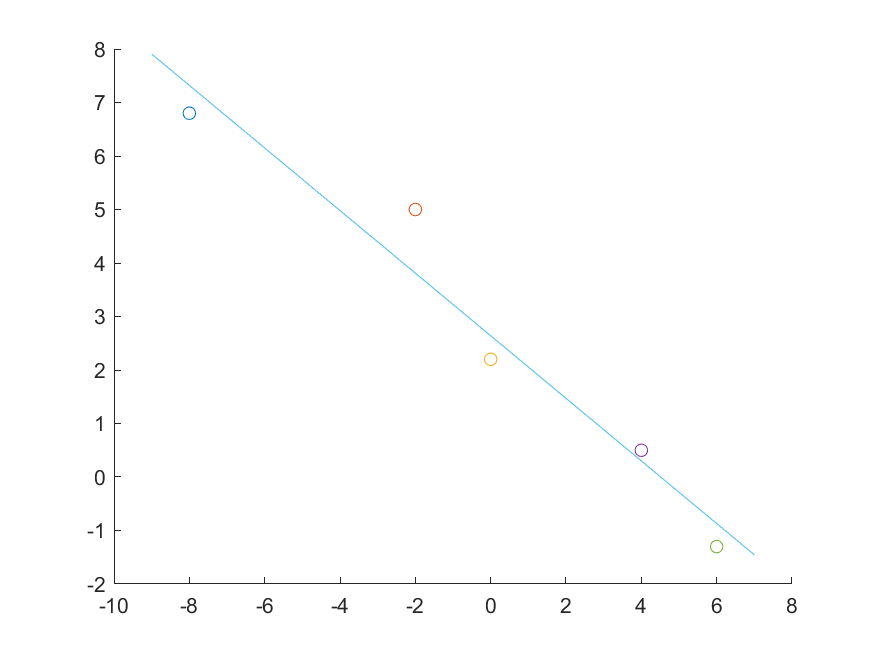
\includegraphics{Images/lineas.png}
        \caption{Gráfica generada por \texttt{lsqGraph.m}}
        \label{pic}
      \end{figure}

      De la gráfica es posible observar que, para la función calculada, esta efectivamente se ajusta lo mejor posible hacia los valores que datos para realizar el cálculo de la misma. De la misma manera, esto nos permite ver la tendencia que los datos tienen a tomar a medida que estos van moviendo a través del eje positivo de las x.

    \end{enumerate}

    \item Interprendo
    
    \begin{enumerate}
      \item Como manera inicial, se pide encontrar la línea de mínimos cuadrados para realizar unas aproximaciones a las leyes de Kepler. Con el fin de realizar esto, se nos da la siguiente ecuación:

      \begin{center}
        \begin{math}
          T^2 = C R^3
        \end{math}
      \end{center}

      A partir de esta, podemos transformarla, aplicando logaritmos, en algo más parecido a la típica forma de una recta:

      \begin{center}
        \begin{math}
          \ln (T^2) = \ln (CR^3)
        \end{math}

        \begin{math}
          \ln(T^2) = \ln(R^3) + \ln(C) 
        \end{math}
      \end{center}

      Con esto, podemos realizar el cálculo de lo que realmente serían los valores de $x_k$ y $y_k$. Este proceso se realizó dentro del script \texttt{keplerRunner.m} en el cual se realiza tanto el cálculo de los valores como la recta resultante.

      \begin{lstlisting}
datosPlanetarios = [87.97 57.91e6;
                    224.70 108.70e6;
                    365.26 149.60e6;
                    686.98 227.92e6;
                    4332.59 778.57e6;
                    10759.22 1433.53e6;
                    30685.40 2872.46e6;
                    60189.00 4495.06e6;];

datosAlterados = [log(datosPlanetarios(:,2).^3), log(datosPlanetarios(:,1).^2)];

lsquare(datosAlterados)
      \end{lstlisting}

      Tras la ejecución de esta, podemos observar en la consola la función resultante para los valores dados como datos.

      \begin{lstlisting}
ans =

(562958924640903*x)/562949953421312 - 3143657320373185/70368744177664
      \end{lstlisting}

      De esto, podemos observar que, a diferencia de como era de esperarse, la función de línea de mínimos cuadrados, aunque tiene algunas ligeras diferencias en lo que se considera como el coeficiente de nuestra variable x. Esto quiere decir que, para los datos dados, la relación aunque proporcional, no es exactamente 1:1. Esto puede deberse principalmente por precisión en los decimales en los radios y los días que no son absolutamente precisos.

      \item Con el de realizar un bosquejo de la ecuación resultante, junto con los datos dados, se creó el script \texttt{planetScript.m} el cual generaba la respectiva gráfica.
      
      \begin{lstlisting}
syms x

temp = (562958924640903*x)/562949953421312 - 3143657320373185/70368744177664;
f = matlabFunction(temp);

dom = linspace(40, 70);

scatter(log((57.91e6)^3), log(87.97^2))
hold on
scatter(log((108.70e6)^3), log(224.70^2))
hold on
scatter(log((149.60e6)^3), log(365.26^2))
hold on
scatter(log((227.92e6)^3), log(686.98^2))
hold on
scatter(log((778.57e6)^3), log(4332.59^2))
hold on
scatter(log((1433.53e6)^3), log(10759.22^2))
hold on
scatter(log((2872.46e6)^3), log(30685.40^2))
hold on
scatter(log((4495.06e6)^3), log(60189.00^2))
hold on
text(log((57.91e6)^3)-4, log(87.97^2), 'Mercurio')
hold on
text(log((108.70e6)^3)-4, log(224.70^2), 'Venus')
hold on
text(log((149.60e6)^3)-4, log(365.26^2), 'Tierra')
hold on
text(log((227.92e6)^3)-4, log(686.98^2), 'Marte')
hold on
text(log((778.57e6)^3)-4, log(4332.59^2), 'Jupiter')
hold on
text(log((1433.53e6)^3)-4, log(10759.22^2), 'Saturno')
hold on
text(log((2872.46e6)^3)-4, log(30685.40^2), 'Urano')
hold on
text(log((4495.06e6)^3)-4, log(60189.00^2), 'Neptuno')
hold on
plot(dom, f(dom));
      \end{lstlisting}

      El resultado de esto, es la figura \ref{planetas} que muestra los valores tras la respectiva transformación de los datos para la realización del cálculo de la línea de mínimos cuadrados.

      \begin{figure}[H]
        \centering
        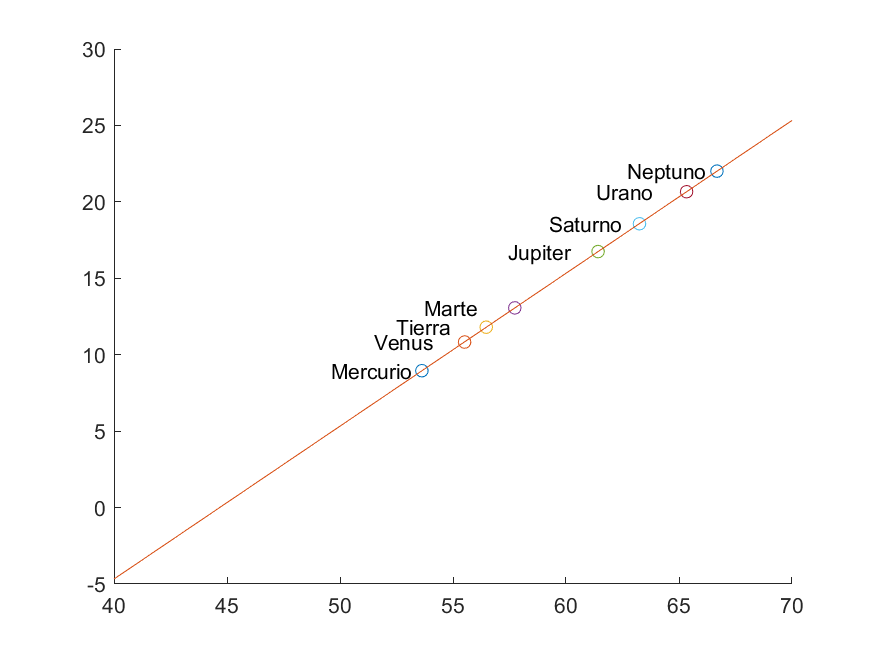
\includegraphics{Images/planetas.png}
        \caption{Relación de la línea de mínimos cuadrados y los datos correspondientes}
        \label{planetas}
      \end{figure}

      \item finalmente, se nos pide realizar una aproximación a la constante gravitacional universal que se tomó a partir de la ecuación resultante calculada con la función \texttt{lsquare(pointMatrix)}. Para realizar esto, debemos tomar el valor B de la ecuación y realizar el despeje respectivo:
      
      \begin{center}
        \begin{math}
          B = \ln(C)
        \end{math}

        \begin{math}
          \displaystyle -\frac{3143657320373185}{70368744177664} = \ln(C)
        \end{math}
        
        \begin{math}
          \displaystyle e^{-\frac{3143657320373185}{70368744177664}} = C
        \end{math}

        \begin{math}
          \displaystyle e^{-\frac{3143657320373185}{70368744177664}} = \frac{4\pi^2}{GM}
        \end{math}

        \begin{math}
          \displaystyle G = \frac{4\pi^2}{e^{-\frac{3143657320373185}{70368744177664}} M}
        \end{math}

        \begin{math}
          \displaystyle G = \frac{4\pi^2}{e^{-\frac{3143657320373185}{70368744177664}} \cdot 1.989 \times 10^{30}}
        \end{math}

        \begin{math}
          \displaystyle G = 5.0052017782\times 10^{-10}
        \end{math}
      \end{center}

      Hay que denotar que, para este caso, existe una gran diferencia en cuanto a la constante universal gravitacional calculada y la establecida por Newton, pero, como se había indicado antes, esto puede deberse a la falta de precisión en los decimales dados como datos para el cálculo de la línea.

    \end{enumerate}

\end{enumerate}

\newpage

\section{Anexos}

\texttt{lsquare(pointMatrix)}.
      
      \begin{lstlisting}
function output = lsquare(pointMatrix)

    syms x

    output = NaN;

    [vS, hS] = size(pointMatrix);

    if hS == 2 && vS > 1
        sumX = sum(pointMatrix(:,1));
        sumY = sum(pointMatrix(:,2));
        sumX2 = sum(pointMatrix(:,1).^2);
        sumXY = sum(pointMatrix(:,1).*pointMatrix(:,2));
        N = vS;

        coTrix = [sumX2, sumX; sumX, N];
        anTrix = [sumXY; sumY];

        vals = linsolve(coTrix, anTrix);

        output = vals(1)*x+vals(2);
    end
end
      \end{lstlisting}

      \texttt{squareRunner.m}

      \begin{lstlisting}
vals = [-8 6.8; -2 5.0; 0 2.2; 4 0.5; 6 -1.3];

f = lsquare(vals)
f = matlabFunction(f);
[n, ~] = size(vals);

funVal = [];
for index = 1:n
    funVal = [funVal; f(vals(index,1))];
end

funVal
    \end{lstlisting}

    \texttt{lsqGraph.m}

    \begin{lstlisting}
f = @(x) 66/25 - (117*x)/200;
xk = linspace(-9, 7);
scatter(-8, 6.8)
hold on
scatter(-2, 5.0) 
hold on
scatter(0, 2.2) 
hold on
scatter(4, 0.5) 
hold on
scatter(6, -1.3)
hold on 
plot(xk, f(xk))
    \end{lstlisting}

    \texttt{keplerRunner.m}

    \begin{lstlisting}
datosPlanetarios = [87.97 57.91e6;
                    224.70 108.70e6;
                    365.26 149.60e6;
                    686.98 227.92e6;
                    4332.59 778.57e6;
                    10759.22 1433.53e6;
                    30685.40 2872.46e6;
                    60189.00 4495.06e6;];

datosAlterados = [log(datosPlanetarios(:,2).^3), log(datosPlanetarios(:,1).^2)];

lsquare(datosAlterados)
    \end{lstlisting}

    \texttt{planetScript.m}

    \begin{lstlisting}
syms x

temp = (562958924640903*x)/562949953421312 - 3143657320373185/70368744177664;
f = matlabFunction(temp);

dom = linspace(40, 70);

scatter(log((57.91e6)^3), log(87.97^2))
hold on
scatter(log((108.70e6)^3), log(224.70^2))
hold on
scatter(log((149.60e6)^3), log(365.26^2))
hold on
scatter(log((227.92e6)^3), log(686.98^2))
hold on
scatter(log((778.57e6)^3), log(4332.59^2))
hold on
scatter(log((1433.53e6)^3), log(10759.22^2))
hold on
scatter(log((2872.46e6)^3), log(30685.40^2))
hold on
scatter(log((4495.06e6)^3), log(60189.00^2))
hold on
text(log((57.91e6)^3)-4, log(87.97^2), 'Mercurio')
hold on
text(log((108.70e6)^3)-4, log(224.70^2), 'Venus')
hold on
text(log((149.60e6)^3)-4, log(365.26^2), 'Tierra')
hold on
text(log((227.92e6)^3)-4, log(686.98^2), 'Marte')
hold on
text(log((778.57e6)^3)-4, log(4332.59^2), 'Jupiter')
hold on
text(log((1433.53e6)^3)-4, log(10759.22^2), 'Saturno')
hold on
text(log((2872.46e6)^3)-4, log(30685.40^2), 'Urano')
hold on
text(log((4495.06e6)^3)-4, log(60189.00^2), 'Neptuno')
hold on
plot(dom, f(dom));
    \end{lstlisting}
\end{document}


